% LaTeX mintafĂĄjl szakdolgozat ĂŠs diplomamunkĂĄknak az
% SZTE Informatikai Tanszekcsoportja ĂĄltal megkĂśvetelt
% formai kĂśvetelmĂŠnyeinek megvalĂłsĂ­tĂĄsĂĄhoz
% Modositva: 2011.04.28 Nemeth L. Zoltan
% A fájl használatához szükséges a magyar.ldf 2005/05/12 v1.5-ös vagy későbbi verziója
% ez letölthető a http://www.math.bme.hu/latex/ weblapról, a magyar nyelvű szedéshez
% Hasznos informĂĄciĂłk, linekek, LaTeX leirasok a www.latex.lap.hu weboldalon vannak.
%


\documentclass[12pt]{report}

%Magyar nyelvi támogatás (Babel 3.7 vagy későbbi kell!)
\def\magyarOptions{defaults=hu-min}
\usepackage[magyar]{babel}

%Az ĂŠkezetes betĹąk hasznĂĄlatĂĄhoz:
\usepackage{t1enc}% ĂŠkezetes szavak automatikus elvĂĄlasztĂĄsĂĄhoz
\usepackage[latin2]{inputenc}% ĂŠkezetes szavak bevitelĂŠhez

% A formai kovetelmenyekben megkĂśvetelt Times betĹątĂ­pus hasznalata:
\usepackage{times}

%Az AMS csomagjai
\usepackage{amsmath}
\usepackage{amssymb}
\usepackage{amsthm}

%A fejlĂŠc lĂĄblĂŠcek kialakĂ­tĂĄsĂĄhoz:
\usepackage{fancyhdr}

%TermĂŠszetesen tovĂĄbbi csomagok is hasznĂĄlhatĂłk,
%pĂŠldĂĄul ĂĄbrĂĄk beillesztĂŠsĂŠhez a graphix ĂŠs a psfrag,
%ha nincs rĂĄjuk szĂźksĂŠg termĂŠszetesen kihagyhatĂłk.
\usepackage{graphicx}
\usepackage{psfrag}

%TĂŠtelszerĹą kĂśrnyezetek definiĂĄlhatĂłk, ezek most fejezetenkent egyutt szamozodnak, pl.
\newtheorem{tĂŠt}{TĂŠtel}[chapter]
\newtheorem{defi}[tĂŠt]{DefinĂ­ciĂł}
\newtheorem{lemma}[tĂŠt]{Lemma}
\newtheorem{åll}[tÊt]{Állítås}
\newtheorem{kĂśv}[tĂŠt]{KĂśvetkezmĂŠny}

%Ha a megjegyzések és a példak szövegét nem akarjuk dőlten szedni, akkor
%az alábbi parancs után kell őket definiální:
\theoremstyle{definition}
\newtheorem{megj}[tĂŠt]{MegjegyzĂŠs}
\newtheorem{pld}[tĂŠt]{PĂŠlda}

%MargĂłk:
\hoffset -1in
\voffset -1in
\oddsidemargin 35mm
\textwidth 150mm
\topmargin 15mm
\headheight 10mm
\headsep 5mm
\textheight 237mm




\begin{document}

%A FEJEZETEK KEZDŐOLDALAINAK FEJ ES LÁBLÉCE:
%a plain oldalstĂ­lust kell ĂĄtdefiniĂĄlni, hogy ott ne legyen fejlĂŠc:
\fancypagestyle{plain}{%
%ez mindent tĂśrĂśl:
\fancyhf{}
% a lĂĄblĂŠcbe jobboldalra kerĂźljĂśn az oldalszĂĄm:
\fancyfoot[R]{\thepage}
%elvĂĄlasztĂł vonal sem kell:
\renewcommand{\headrulewidth}{0pt}
}

%A TÖBBI OLDAL FEJ ÉS LÁBLÉCE:
\pagestyle{fancy}
\fancyhf{}
\fancyhead[L]{Minőségkinyerés borkóstolási adatokból, web és android alkalmazás fejlesztés}
\fancyfoot[R]{\thepage}


%A cĂ­moldalra se fej- se lĂĄblĂŠc nem kell:
\thispagestyle{empty}

\begin{center}
\vspace*{1cm}
{\Large\bf Szegedi TudomĂĄnyegyetem}

\vspace{0.5cm}

{\Large\bf Informatikai TanszĂŠkcsoport}

\vspace*{3.8cm}


{\LARGE\bf Minőségkinyerés borkóstolási adatokból, web és android alkalmazás fejlesztés}


\vspace*{3.6cm}

{\Large Szakdolgozat}
% vagy {\Large Szakdolgozat}

\vspace*{4cm}

%Értelemszerűen megváltoztatandó:
{\large
\begin{tabular}{c@{\hspace{4cm}}c}
\emph{Készítette:}     &\emph{Témavezető:}\\
\bf{Varga TamĂĄs}  &\bf{Dr. Csendes Tibor}\\
Programtervező Informatikus     &tanszékvezető egyetemi tanár\\
hallgatĂł&
\end{tabular}
}

\vspace*{2.3cm}

{\Large
Szeged
\\
\vspace{2mm}
2015
}
\end{center}


%A tartalomjegyzĂŠk:
\tableofcontents

%A \chapter* parancs nem ad a fejezetnek sorszĂĄmot
\chapter*{FeladatkiĂ­rĂĄs}
%A tartalomjegyzĂŠkben mĂŠgis szerepeltetni kell, mint szakasz(section) szerepeljen:
\addcontentsline{toc}{section}{FeladatkiĂ­rĂĄs}

A témavezető által megfogalmazott feladatkiírás. Önálló oldalon szerepel.

\chapter*{Tartalmi ĂśsszefoglalĂł}
\addcontentsline{toc}{section}{Tartalmi ĂśsszefoglalĂł}

A tartalmi összefoglalónak tartalmaznia kell (rövid, legfeljebb egy oldalas, összefüggő megfogalmazásban)
a következőket: a téma megnevezése, a megadott feladat megfogalmazása - a feladatkiíráshoz viszonyítva-,
a megoldĂĄsi mĂłd, az alkalmazott eszkĂśzĂśk, mĂłdszerek, az elĂŠrt eredmĂŠnyek, kulcsszavak (4-6 darab).

Az ĂśsszefoglalĂł nyelvĂŠnek meg kell egyeznie a dolgozat nyelvĂŠvel. Ha a dolgozat idegen nyelven kĂŠszĂźl,
magyar nyelvű tartalmi összefoglaló készítése is kötelező (külön lapon), melynek terjedelmét a TVSZ szabályozza.


\chapter*{BevezetĂŠs}
\addcontentsline{toc}{section}{BevezetĂŠs}

Itt kezdődik a bevezetés, mely nem kap sorszámot.



\chapter{BorkĂłstolĂł algoritmusok}

Ez pedig már az első fejezet, ...

\section{CoHITS}
A CoHITS

%\subsection{Al-al cĂ­m}
%Sőt al-al fejezetek is.

%\subsection{MĂĄsik}
%Na lĂĄssunk egy mĂĄsodikat is.

%\subsection{Harmadik}
%Meg egy harmadikat is.

\section{Hamming}
Hamming

\section{Koszinusz}
Koszinusz

\section{Precedencia}
Precedencia

\section{Összefüggőségi}
Összefüggőségi

\section{PozĂ­ciĂł szerinti}
PozĂ­ciĂł szerinti

\chapter{A weboldal}

\section{IterĂĄciĂłk}

\section{PHP}

\section{JavaScript}

\section{Grafikonok}
\subsection{Google Charts}
\subsection{Charts.js}

\section{Statikus tartalom}
\subsection{index.html - Főoldal}
\subsection{borkostolasEredmenyek.html - EredmĂŠnyek}
\subsection{modszerek.html - MĂłdszerek}
\subsection{kapcsolat.html - Kapcsolat}

\section{Dinamikus tartalom}
\subsection{RegisztrĂĄciĂł}
\subsection{BejelentkezĂŠs}
\subsection{demo.html - DemĂł}

\chapter{A mobil alkalmazĂĄs}
Androd alkalmazĂĄs fejlesztĂŠs

\section{Android}
Android

\chapter{A weboldal ĂŠs a mobil alkalmazĂĄs ĂśsszefĹązĂŠse}
A weboldal ĂŠs a mobil alkalmazĂĄs ĂśsszefĹązĂŠse

\chapter{TesztelĂŠs}
\section{Regisztrációs és bejelentkeztető rendszer}
\section{Demo adatkezelésének ellenőrzése}
\section{Algoritmusok ellenőrzése kis adatokon}
\section{Algoritmusok ellenőrzése ismert eredményekkel}

\chapter{Összefoglalás}

\chapter{Egyebek}
\section{VerziĂł kezelĂŠs}

\section{KĂśrnyezetek}
SublimeText3 - linterek\\

AndroidStudi

%\begin{tĂŠt}
%\label{tĂŠt-alap}
%Ez itt egy tĂŠtel.
%\end{tĂŠt}

%%A bizonyĂ­tĂĄs \begin{proof} ĂŠs \end{proof} kĂśzĂŠ kerĂźl:
%\begin{proof}
%Ez pedig a bizonyĂ­tĂĄsa, melyben szerepel egy kĂŠplet:
%\begin{equation}
%\begin{split}
%E^{\text{globĂĄlis}} &= \text{tĂŠt}_1\cdot E_1^{\text{elemi}}+\text{tĂŠt}_2\cdot
%E_2^{\text{elemi}}+\ldots+\text{tĂŠt}_n\cdot E_n^{elemi} \\
%&=E^{\text{elemi}}\left(\text{tĂŠt}_1+\text{tĂŠt}_2+\ldots+\text{tĂŠt}_n\right)\\
%&=E^{\text{elemi}}\cdot\text{ĂśssztĂŠt}
%\end{split}
%\end{equation}
%A második egyenlőségnél azt használtunk ki, hogy ...
%
%Ezzel a bizonyĂ­tĂĄst befejeztĂźk.
%\end{proof}

%\begin{defi}
%\label{def-pelda}
%Ez egy definĂ­ciĂł. SzĂĄmozĂĄsa a tĂŠtelekkel egyĂźtt tĂśrtĂŠnik.
%\end{defi}

%\begin{ĂĄll}
%A követekező négy állítás egymással ekvivalens:
%\label{ĂĄll-ekvivalencia}
%  \begin{itemize}
%  \item[(i)] $M$ ĂŠs $N$ gyengĂŠn ekvivalensek.
%  \item[(ii)] Minden $n$
%  nemnegatĂ­v egĂŠsz szĂĄmra $|L_{M}\cap \Sigma_{1}^{n}|=|L_{N}\cap \Sigma_{2}^{n}|$ teljesĂźl.
%  \item[(iii)] Minden $n$ nemnegatĂ­v egĂŠsz szĂĄm esetĂŠn
%   lĂŠtezik
%  $ \pi_{n}: L_{M}\cap \Sigma_{1}^{n} \rightarrow L_{N}\cap \Sigma_{2}^{n} $ kĂślcsĂśnĂśsen egyĂŠrtelmĹą
%  lekĂŠpezĂŠs.
%  \item[(iv)] Minden nemnegatĂ­v $n$-re $x A^{n} y^{T}=x' A'^{n} y'^{T}$.
%  \end{itemize}
%\end{ĂĄll}

%\begin{kĂśv}
%  Ez pedig egy kĂśvetkezmĂŠny.
%\end{kĂśv}

%\begin{pld}
%  Ez lesz a példa, ezt nem szedjük dőlten.
%\end{pld}

%\begin{megj}
%  A fejezetet pedig egy megjegyzĂŠs zĂĄrja.
%\end{megj}


%\section{ListĂĄk}
%
%Ez egy felsorolĂĄs:
%\begin{itemize}
%    \item első
%    \item mĂĄsodik
%      \subitem első
%      \subitem mĂĄsodik
%    \item harmadik
%    \item[$\clubsuit$]  sajĂĄt jel is alkalmazhatĂł
%\end{itemize}
%Ez pedig egy szĂĄmozott lista:
%\begin{enumerate}
%            \item hétfő
%            \item kedd
%            \item szerda
%\end{enumerate}

%OldaltĂśrĂŠst is alkalmazhatunk
\pagebreak


%\section{Egy tĂĄblĂĄzat ĂŠs egy ĂĄbra}
%
%A tĂĄblĂĄzat itt kĂśvetkezik.
%\begin{table}[!h]\label{strategia}
%\caption{PĂŠlda stratĂŠgiatĂĄblĂĄra a Black Jack esetĂŠben}
%\begin{center}
%\begin{tabular}{l||r|r|r|r|r|r|r|r|r|r}
%&ĂĄsz&2&3&4&5&6&7&8&9&10\\
%\hline\hline
%21&n&n&n&n&n&n&n&n&n&n\\
%20&n&n&n&n&n&n&n&n&n&n\\
%19&n&n&n&n&n&n&n&n&n&n\\
%18&n&n&n&n&n&n&n&n&n&n\\
%17&n&n&n&n&n&n&n&n&n&n\\
%16&h&n&n&n&n&n&h&h&b&b\\
%15&h&n&n&n&n&n&h&h&h&b\\
%14&h&n&n&n&n&n&h&h&h&b\\
%13&h&n&n&n&n&n&h&h&h&h\\
%12&h&n&n&n&n&n&h&h&h&h\\
%11&h&D&D&D&D&D&D&D&D&h\\
%\end{tabular}
%\end{center}
%\end{table}
%
%LĂĄssunk egy ĂĄbrĂĄt is!
%\begin{figure}[!h]
%\unitlength 8mm
%\begin{center}
%\begin{picture}(8,6)
%\thicklines
%\multiput(0,1)(0,1){2}{\line(1,0){5}}
%\multiput(3,0)(1,0){2}{\line(0,1){6}}
%\multiput(1,0)(1,0){2}{\line(0,1){1}}
%\multiput(6,0)(1,0){2}{\line(0,1){5}}
%\multiput(0,1)(1,0){3}{\line(0,1){1}}
%\multiput(2,4)(3,0){3}{\line(0,1){1}}
%\multiput(3,0)(0,3){3}{\line(1,0){1}}
%\multiput(6,0)(0,1){4}{\line(1,0){1}}
%\multiput(7,2)(0,1){2}{\line(1,0){1}}
%\multiput(2,4)(0,1){2}{\line(1,0){6}}
%\put(5,1){\line(0,1){1}}
%\put(8,2){\line(0,1){1}}
%\put(1,0){\line(1,0){1}}
%\put(1,1){\makebox(1,1){\(\sphericalangle\)}}
%\put(7,2){\makebox(1,1){\(\$\)}}
%\end{picture}
%\end{center}
%\caption{\label{labirintus}Labirintus bejĂĄrĂĄsa}
%\end{figure}

%laptĂśrĂŠs:
\newpage
%
KĂźlĂśn fĂĄjlban elkĂŠszĂ­tett grafika beillesztĂŠsĂŠt a 
%\ref{abra-automata} ĂĄbra szemlĂŠlteti.
%\begin{figure}[h]
%\centering
%%A psfrag csomag hasznĂĄlatĂĄval a (encapsulated)postcript abra feliratait LaTeX koddal helyettesĂ­thatjĂźk:
%\psfrag{a}[c][c]{$q_0$}
%\psfrag{b}[c][c]{$q_1$}
%\psfrag{c}[c][c]{$q_2$}
%\psfrag{d}[c][c]{$q_3$}
%\psfrag{e}[c][c]{$q_4$}
%\psfrag{f}[c][c]{$q_5$}
%\psfrag{g}[c][c]{$q_6$}
%\psfrag{h}[c][c]{$q_7$}
%\psfrag{0}[c][c]{$a_{0}$}
%\psfrag{9}[c][c]{$a_{9}$}
%\psfrag{3}[c][c]{$a_{3}$}
%\psfrag{12}[c][c]{$a_{12}$}
%\psfrag{15}[c][c]{$a_{15}$}
%%Garfika belillesztese, "scale2 a nagyitas/kicinyites merteke, itt 80%.
%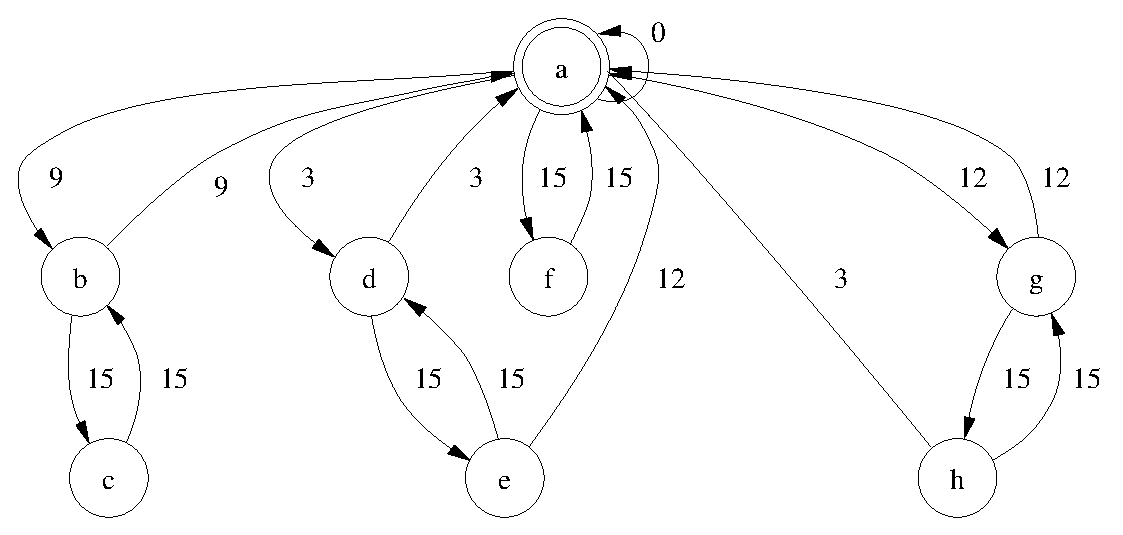
\includegraphics[scale=0.8]{abra.eps}
%\caption{\label{abra-automata} A $4\times m$-es tábla lefedéseinek mátrixreprezentációit felismerő automata}
%\end{figure}


\chapter{FĂźggelĂŠk}

\section{A program forrĂĄskĂłdja}
%A fĂźggelĂŠkbe kerĂźlhetnek a hosszĂş tĂĄblĂĄzatok, vagy mondjuk egy programlista:
%% A verbatim kornyezet hasznalatanal ĂźgyeljĂźnk rĂĄ, hogy az editor a szĂłkĂśzĂśjket ĂĄt ne Ă­rja tab karakterekre!
%\begin{verbatim}
%   while (ujkmodosito[i]<0)
%   {
%      if (ujkmodosito[i]+kegyenletes[i]<0)
%      {
%         j=i+1;
%         while (j<14)
%         if (kegyenletes[i]+ujkmodosito[j]>-1) break;
%         else j++;
%         temp=ujkmodosito[j];
%         for (l=i;l<j;l++) ujkmodosito[l+1]=ujkmodosito[l];
%         ujkmodosito[i]=temp;
%      }
%      i++;
%   }
%\end{verbatim}


\chapter*{Nyilatkozat}
%Egy Ăźres sort adunk a tartalomjegyzĂŠkhez:
\addtocontents{toc}{\ }
\addcontentsline{toc}{section}{Nyilatkozat}
%\hspace{\parindent}

% A nyilatkozat szĂśvege mĂĄs titkos ĂŠs nem titkos dolgozatok esetĂŠben.
% Csak az egyik tipusĂş myilatokzatnak kell a dolgozatban szerepelni
% A ponok helyére az adatok értelemszerűen behelyettesídendők es
% a szakdolgozat /diplomamunka szo megfeleloen kivalasztando.


%A nyilatkozat szövege TITKOSNAK NEM MINŐSÍTETT dolgozatban a következő:
%A pontokkal jelölt szövegrészek értelemszerűen a szövegszerkesztőben és
%nem kézzel helyettesítendők:

\noindent
AlulĂ­rott \makebox[4cm]{\dotfill} szakos hallgatĂł, kijelentem, hogy a dolgozatomat a Szegedi TudomĂĄnyegyetem, Informatikai TanszĂŠkcsoport \makebox[4cm]{\dotfill} TanszĂŠkĂŠn kĂŠszĂ­tettem, \makebox[4cm]{\dotfill} diploma megszerzĂŠse ĂŠrdekĂŠben.

Kijelentem, hogy a dolgozatot mĂĄs szakon korĂĄbban nem vĂŠdtem meg, sajĂĄt munkĂĄm eredmĂŠnye, ĂŠs csak a hivatkozott forrĂĄsokat (szakirodalom, eszkĂśzĂśk, stb.) hasznĂĄltam fel.

TudomĂĄsul veszem, hogy szakdolgozatomat / diplomamunkĂĄmat a Szegedi TudomĂĄnyegyetem Informatikai TanszĂŠkcsoport kĂśnyvtĂĄrĂĄban, a helyben olvashatĂł kĂśnyvek kĂśzĂśtt helyezik el.

\vspace*{2cm}

\begin{tabular}{lc}
Szeged, \today\
\hspace{2cm} & \makebox[6cm]{\dotfill} \\
& alĂĄĂ­rĂĄs \\
\end{tabular}


\vspace*{4cm}





%% Az itrodalomjegyzek keszitheto a BibTeX segedprogrammal:
%\bibliography{diploma}
%\bibliographystyle{plain}

%VAGY "kézzel" a következő módon:

\begin{thebibliography}{9}
%10-nĂŠl kevesebb hivatkozĂĄs esetĂŠn

%\begin{thebibliography}{99}
% 10-nĂŠl tĂśbb hivatkozĂĄs esetĂŠn

\addcontentsline{toc}{section}{IrodalomjegyzĂŠk}

%Elso szerzok vezetekneve alapjan ĂĄbĂŠcĂŠrendben rendezve.


%folyĂłirat cikk: szerzok(k), a folyĂłirat neve kiemelve,
%az evfolyam felkoveren, zarojelben az evszam, vegul az oldalszamok es pont.

%\bibitem{Gischer}
%J. L. Gischer,
%The equational theory of pomsets.
%\emph{Theoret. Comput. Sci.}, \textbf{61}(1988), 199--224.

%kĂśnyv (szerzo(k), a kĂśnyv neve kiemelve, utana a kiado, a kiado szekhelye, az evszam es pont.)

%\bibitem{Pin}
%J.-E. Pin,
%\emph{Varieties of Formal Languages},
%Plenum Publishing Corp., New York, 1986.





\end{thebibliography}




\end{document}
